\documentclass[a4paper, 10pt]{article}

\usepackage[T1]{fontenc}
\usepackage[utf8]{inputenc}
\usepackage[croatian]{babel}
\usepackage{amsmath}
\usepackage{amsfonts}
\usepackage{graphicx} % slike
\usepackage{epstopdf} % eps grafika
\usepackage{listings} % blokovi koda
\usepackage{color}
\usepackage{comment} % blokovi komentara
\usepackage{hyperref}
%\usepackage[nottoc, notbib]{tocbibind} % dodaj popis slika i tablica u toc
\usepackage{lmodern} % bold stil za tt
\usepackage{afterpage}
\usepackage{float} % [H] za figure
\usepackage{indentfirst} % indent u prvom paragrafu sekcije

%\setlength{\parindent}{0in} % bez indenta u novom paragrafu
%\setlength{\parskip}{\baselineskip} % razmak između paragrafa

\hypersetup{
  unicode = true,
  colorlinks = true,
  urlcolor = black, % boja vanjskih linkova
  linkcolor = black, % boja linkova u dokumentu
  citecolor = red % boja citata
}

%\definecolor{lightgray}{gray}{0.92}

\lstset{
   language = Matlab,
   frame = single,
   %backgroundcolor = \color{lightgray},
   basicstyle = \ttfamily,
   showstringspaces = false,
   showspaces = false,
   breaklines = true,
   inputencoding = utf8, % hr slova
   extendedchars = true, % hr slova
   morekeywords = {ones, mod, randi, rng, saveas}
}

% hrvatska slova u blokovima koda
\lstset{
    literate=%
    {ć}{{\'c}}1
    {č}{{\v{c}}}1
    {đ}{{\dj{}}}1
    {š}{{\v{s}}}1
    {ž}{{\v{z}}}1
    {Ć}{{\'C}}1
    {Č}{{\v{C}}}1
    {Đ}{{\DJ{}}}1
    {Š}{{\v{S}}}1
    {Ž}{{\v{Z}}}1
}

\begin{comment}
\title{Kratki uvod u MATLAB}
\author{Edvin Močibob}
\date{\today}
\end{comment}

\newcommand{\spec}[1]{\texttt{#1}}

\begin{document}

%\maketitle

\begin{titlepage}
\newcommand{\HRule}{\rule{\linewidth}{0.5mm}}
\begin{center}

% Vrh stranice
\textsc{\LARGE Sveučilište u Rijeci}\\[0.5cm]
\textsc{\Large Odjel za informatiku}\\[2.5cm]

% Naslov
\HRule \\[0.4cm]
%{\huge Kratki uvod u MATLAB}\\[0.1cm]
{\huge \bfseries Kratki uvod u MATLAB}\\[0.1cm]

\HRule \\[1.5cm]

% Autor
\begin{minipage}{0.5\textwidth}
	\begin{center}
		\large
		\textsc{\Large Edvin Močibob}\\[0.1cm]
		\texttt{\href{mailto:edvin.mocibob@gmail.com}{edvin.mocibob@gmail.com}}
	\end{center}
\end{minipage}

\vfill
% Dno naslovne
{\large \today}
\end{center}
\end{titlepage}

%\newpage\null\thispagestyle{empty}\addtocounter{page}{-1}\newpage % prazna stranica

\tableofcontents
\clearpage

%%%%%%%%%%%%%%%%%%%%%%%%%%%%%%%%%%%%%%%%%%%%%%%%%%%%%%%%
%%%%%%%%%%%%%%%%%%%%%%%%%%%%%%%%%%%%%%%%%%%%%%%%%%%%%%%%
%%%%%%%%%%%%%%%%%%%%%%%%%%%%%%%%%%%%%%%%%%%%%%%%%%%%%%%%

\section*{Uvod}
\addcontentsline{toc}{section}{Uvod}

MATLAB (\emph{\textbf{mat}rix \textbf{lab}oratory}) označava programski jezik i interaktivno okruženje za vršenje programskih izračuna.
Popularan je alat u matematici, inženjerstvu i znanosti.
Osim u akademskom okruženju ima široku primjenu i u industriji.
Podržan je za više popularnih operacijskih sustava kao Microsoft Windows, GNU/Linux i Mac OS X.
Više informacija dostupno je na Wikipediji\footnote{\texttt{\href{https://en.wikipedia.org/wiki/MATLAB}{www.wikipedia.org/wiki/MATLAB}}} i službenoj stranici\footnote{\texttt{\href{http://www.mathworks.com/products/matlab/}{www.mathworks.com/products/matlab/}}}.

U nastavku slijedi kratki uvod u sintaksu MATLAB-a prezentiran (većinom) kroz primjere\footnote{Prezentirani kod testiran je u MATLAB verziji R2014a na Windows 7 operacijskom sustavu.}.
MATLAB ima kvalitetnu dokumentaciju sa primjerima i preporučeno je njezino korištenje uz ovaj dokument.
Blokovi koda se neće opširno objašnjavati te pretpostavlja se da čitatelj ima neko bazično znanje iz programiranja.

Kontaktiranje autora u vezi grešaka u tekstu i unaprjeđenja sadržaja preko email adrese na naslovnoj stranici.
\LaTeX\ kod kojim je generiran ovaj dokument trenutno se nalazi na \texttt{\href{https://github.com/emocibob/Kratki-uvod-u-MATLAB}{www.github.com/emocibob/Kratki-uvod-u-MATLAB}} pod MIT licencom.

\clearpage

%%%%%%%%%%%%%%%%%%%%%%%%%%%%%%%%%%%%%%%%%%%%%%%%%%%%%%%%
%%%%%%%%%%%%%%%%%%%%%%%%%%%%%%%%%%%%%%%%%%%%%%%%%%%%%%%%
%%%%%%%%%%%%%%%%%%%%%%%%%%%%%%%%%%%%%%%%%%%%%%%%%%%%%%%%

\section{Osnove}

Jednolinijski komentari počinju sa \spec{\%}.
Izlaz naredbe neće se prikazati ako naredba završi sa \spec{;}.

\begin{lstlisting}
x = 5; % inicijaliziraj varijablu x na 5
\end{lstlisting}

Brojeve i vrijednosti varijabla možemo ispisati u komandnoj liniji samim njihovim navođenjem.

\begin{lstlisting}
10 % ispiši broj 10
x % ispiši vrijednost spremljenu u x
\end{lstlisting}

Slijedi generiranje vektora koji sadrži $4$ vrijednosti od $1$ do $10$ (granice uključne).
Sve susjedne vrijednosti su međusobno jednako udaljene.

\begin{lstlisting}
linspace(1, 10, 4) % rezultat sadrži 1, 4, 7 i 10
\end{lstlisting}

Isti rezultat dobijemo sljedećom naredom.
Ovdje ne odredimo eksplicitno broj elementa nego inkrement\footnote{Ako je inkrement $1$ možemo izostaviti drugi argument, tj.\ pišemo \spec{[a:b]} za sve cijele brojeve od \spec{a} do \spec{b}.} za svaki sljedeći element -- u ovom slučaju $3$.

\begin{lstlisting}
[1:3:10]
\end{lstlisting}

Slijedi primjer indeksiranja vektora i matrica (više u sekciji \nameref{sec:matrice}).
Valja zapamtiti da indeksi elementa počinju od $1$.

\begin{lstlisting}
v = [100:150]; % cijeli brojevi od 100 do 150
v(1) % prvi element
v(1:10) % prvih 10 elemenata
v(2:2:50) % neparni elementi
v([9 9 9]) % tri puta vrati 9. element
\end{lstlisting}

U sljedećem kodu potencira se broj i vektor.
Primijetimo \spec{.} tj.\ operator točke.
Ako je on ispred nekog drugog operatora, drugi operator će izvršiti izračun element po element (tzv.\ \emph{pointwise} operacija\footnote{Tako nam je, na primjer, bitno koristimo li \spec{.*} ili samo \spec{*} kod množenja matrica.
Primjeri u sekciji \nameref{sec:matrice}.}).

\begin{lstlisting}
a = 5
b = [1, 2, 3, 4]
a .^ 3 % 125
b .^ 3 % izlazni vektor sadrži 1, 8, 27 i 64
\end{lstlisting}

MATLAB će brojeve sa puno znamenki zapisati u znanstvenom formatu.
U primjeru je tim formatom spremljen broj $2.1 \times 10^{-8}$.

\begin{lstlisting}
k = 2.1e-8
\end{lstlisting}

Duže naredbe je zbog preglednosti moguće napisati u više linija sa tri točke.

\begin{lstlisting}
n = 1 - 1/12 + 1/123 - 1/1234 + 1/12345 - 1/123456 ...
    + 1/1234567 - 1/12345678 + 1/123456789
\end{lstlisting}

Naredba \spec{lookfor} služi za pretraživanje funkcija iz komandne linije.
Pretraživanje može potrajati pošto MATLAB ima bogatu biblioteku funkcija.

\begin{lstlisting}
lookfor label
\end{lstlisting}

Pristup dokumentaciji za određenu funkciju može se ostvariti iz komandne linije sa \spec{help}.

\begin{lstlisting}
help help
\end{lstlisting}

Cijeli radni prostor može se obrisati narednom \spec{clear} (bez argumenata), dok \spec{clc} služi za brisanje sadržaja komandne linije.
Pojedinačne varijable iz radnog prostora brišemo tako ih navodimo nakon \spec{clear}.

\begin{lstlisting}
clear a b
\end{lstlisting}
Slijedi primjer spremanja radne površine (\emph{workspace}) koristeći \spec{save}. Radna površina biti će spremljena u datoteci pod imenom \spec{vjezba1\_data.mat}.

\begin{lstlisting}
save('vjezba1_data')
\end{lstlisting}

Relacijski operatori u MATLAB-u su sljedeći: \spec{==} je jednako, \spec{<} manje, \spec{>} veće, \spec{<=} manje ili jednako, \spec{>=} veće ili jednako, \spec{\textasciitilde=} različito od.

Modulo operator\footnote{Ostatak cjelobrojnog dijeljenja.} implementiran je funkcijom \spec{mod}.

\begin{lstlisting}
ostatak = mod(29, 3) % daje 2
\end{lstlisting}

Dolje je naveden primjer\footnote{Argument za obje funkcije, tj.\ rezultat \spec{v > 1}, je vektor sa \emph{true}/\emph{false} ($1$/$0$) vrijednostima za pojedine elemente \spec{v}.}
za MATLAB funkcije \spec{any} (da li je ikoji element različit od $0$) i \spec{all} (da li su svi elementi različiti od $0$).

\begin{lstlisting}
v = [1.5 0.9 0.7 0.12 0.1 0.05];
any(v > 1) % ikoji element veći od 1? true
all(v > 1) % svi elementi veći od 1? false
\end{lstlisting}

Za logičke operatore koriste se \spec{\&} (logičko i), \spec{|} (logičko ili) i \spec{\textasciitilde} (komplement).

%%%%%%%%%%%%%%%%%%%%%%%%%%%%%%%%%%%%%%%%%%%%%%%%%%%%%%%%
%%%%%%%%%%%%%%%%%%%%%%%%%%%%%%%%%%%%%%%%%%%%%%%%%%%%%%%%
%%%%%%%%%%%%%%%%%%%%%%%%%%%%%%%%%%%%%%%%%%%%%%%%%%%%%%%%

\section{Matrice}
\label{sec:matrice}

Generiranje $2 \times 3$ matrice koja sadrži samo jedinice.

\begin{lstlisting}
ones(2, 3)
\end{lstlisting}

Inicijalizacija matrice \spec{A} dimenzija $3 \times 4$.

\begin{lstlisting}
A = [1 2 3 4; 10 20 30 40; 100 200 300 400]
\end{lstlisting}

\pagebreak % manualno počni novu stranicu

Transponiranje \spec{A}.
\begin{lstlisting}
A'
\end{lstlisting}

Zbroj elemenata \spec{A} po stupcima.

\begin{lstlisting}
sum(A) % izlaz 1x4 matrica
\end{lstlisting}

Zbroj svih elemenata.

\begin{lstlisting}
sum(sum(A))
\end{lstlisting}

Najveći element iz \spec{A}.

\begin{lstlisting}
max(max(A))
\end{lstlisting}

Najmanji elementi iz pojedinih redaka.

\begin{lstlisting}
min(A, [], 2) % min traži po 2. dimenziji - recima
\end{lstlisting}

Matrica tipa \emph{logical} koja prikazuje koji su elementi \spec{A} veći od $30$.
Izlaz ima iste dimenzije kao \spec{A}, na mjesta elemenata većih od $30$ nalazi se $1$ (\emph{true}) a na ostalim $0$ (\emph{false}).

\begin{lstlisting}
A > 30
\end{lstlisting}

Broj elemenata \spec{A} većih od $30$.

\begin{lstlisting}
sum(sum(A > 30))
\end{lstlisting}

Vrati matricu \spec{P} (tipa \emph{logical}) koja sadrži na kojim mjestima u \spec{A} se nalaze parni brojevi.
Nakon toga ispiši te parne brojeve iz {A}.

\begin{lstlisting}
P = mod(A, 2) == 0;
A(P)
\end{lstlisting}

Matrica \spec{B} koja sadrži elemente \spec{A} povećane za $10$.

\begin{lstlisting}
B = A + 10
\end{lstlisting}

Pojedinim elementima \spec{A} možemo pristupiti sa \spec{A(i, j)} gdje je \spec{i} redak a \spec{j} stupac elementa.
Za raspone koristimo \spec{:}.
Prisjetimo se, indeksiranje počinje od $1$.

\begin{lstlisting}
A(2, 1) % element u drugom retku i prvom stupcu
A(2, :) % drugi redak
A(:, 3:4) % treći i četvrti stupac
\end{lstlisting}

Uvećaj treći stupac 10 puta.

\begin{lstlisting}
A(:, 3) = A(:, 3) * 10;
\end{lstlisting}

Nova matrica kojoj je osim elementa \spec{A} (dimenzije $3 \times 4$) dodan još jedan redak.
Moguće koristiti i \spec{vertcat}\footnote{\spec{vertcat(A, [-1 -2 -3 -4])}}.

\begin{lstlisting}
[A; -1 -2 -3 -4]
\end{lstlisting}

Nova matrica kojoj je osim elementa \spec{A} (dimenzije $3 \times 4$) dodan još jedan stupac.
Moguće koristiti i \spec{horzcat}\footnote{\spec{horzcat(A, [5; 55; 555])}}.

\begin{lstlisting}
[A [5; 55; 555]]
\end{lstlisting}

Jedinična matrica\footnote{Sadrži jedinice na dijagonali.} \spec{B} istih dimenzija kao \spec{A}.

\begin{lstlisting}
B = eye(size(A))
\end{lstlisting}

Inicijaliziraj i zatim matrično pomnoži matrice \spec{C} i \spec{D}.

\begin{lstlisting}
C = [1 2; 3 4];
D = [10 20; 30 40];
C * D
\end{lstlisting}

Množenje matrica \spec{C} i \spec{D} po elementima.

\begin{lstlisting}
C .* D
\end{lstlisting}

Primjer pretvaranja matrice u vektor.

\begin{lstlisting}
A(:)
\end{lstlisting}

%%%%%%%%%%%%%%%%%%%%%%%%%%%%%%%%%%%%%%%%%%%%%%%%%%%%%%%%
%%%%%%%%%%%%%%%%%%%%%%%%%%%%%%%%%%%%%%%%%%%%%%%%%%%%%%%%
%%%%%%%%%%%%%%%%%%%%%%%%%%%%%%%%%%%%%%%%%%%%%%%%%%%%%%%%

\section{Polja ćelija}

Matrice ne mogu sadržavati istovremeno različite tipove podataka (npr.\ brojeve i tekst).
Kada imamo potrebu za tim možemo koristiti polja ćelija (\emph{cell arrays}).

Inicijaliziacija se može izvršiti pomoću vitičastih zagrada.
Što se dimenzija tiče, svi reci moraju imati isti broj elemenata.
U primjeru vidimo da polja ćelija mogu sadržavati druga polja ćelija.

\begin{lstlisting}
C = {'Tekst', 2, {'XYZ', 111}; 4, 5, 10}
\end{lstlisting}

Referenciranje ćelija moguće je pomoću običnih zagrada (gdje se pristupa ćelijama) ili pomoću vitičastih zagrada (gdje se pristupa sadržaju ćelija).

U primjeru prvo pristupamo drugom retku polja \spec{C} i zatim pristupamo vrijednostima istog retka.

\begin{lstlisting}
C(2, :)
C{2, :}
\end{lstlisting}

Prazna ćelija dimenzija $0 \times 0$ može se inicijalizirati na sljedeći način.

\begin{lstlisting}
C2 = {}
\end{lstlisting}

Slijedi primjer u kojem se dodaje element u postojeće polje ćelija.
Dimenzije polja će se automatski povećati ako se referencira ćelija izvan postojećih dimenzija.

\begin{lstlisting}
C2{4, 4} = 9
\end{lstlisting}

Samo povećanje dimenzija bez dodavanja ikakve nove vrijednosti vrši se na sljedeći način.

\begin{lstlisting}
C2{5, 6} = []
\end{lstlisting}

Naredba \spec{cell2mat} se koristi za pretvaranje polja ćelija (ili samo djela polja ćelija) u obični vektor tj.\ matricu.
Uvjet je da svi elementi koji se pretvaraju budu istog tipa.

Sljedeća naredba pretvara drugi redak polja ćelija \spec{C} u vektor\footnote{Isti efekt bi postigla naredba \spec{[C\{2, :\}]}.}.

\begin{lstlisting}
cell2mat(C(2, :))
\end{lstlisting}

%%%%%%%%%%%%%%%%%%%%%%%%%%%%%%%%%%%%%%%%%%%%%%%%%%%%%%%%
%%%%%%%%%%%%%%%%%%%%%%%%%%%%%%%%%%%%%%%%%%%%%%%%%%%%%%%%
%%%%%%%%%%%%%%%%%%%%%%%%%%%%%%%%%%%%%%%%%%%%%%%%%%%%%%%%

\section{Grananja i petlje}

Slijedi primjer sa sintaksom za \spec{if} grananje.

\begin{lstlisting}
n = 9;
if mod(n, 2) == 0
    disp('Broj paran.')
else
    disp('Broj neparan.')
end
\end{lstlisting}

Ispiši \spec{for} petljom brojeve od $1$ do $10$ (granice uključne).

\begin{lstlisting}
for i = 1:10
    i
end
\end{lstlisting}

Ista stvar u \spec{while} petlji.

\begin{lstlisting}
i = 1;
while i <= 10
    i
    i = i + 1;
end
\end{lstlisting}

Ispiši \spec{for} petljom svaki drugi broj od $1$ do $10$ (tj.\ ispiši $1$, $3$, $5$, $7$ i $9$).

\begin{lstlisting}
for i = 1:2:10
    i
end
\end{lstlisting}

Primjer prolaska kroz vektor \spec{for} petljom.

\begin{lstlisting}
for el = [5 2 36 1 9]
   el
end
\end{lstlisting}

\pagebreak

Sljedećim blokom koda\footnote{Primjer služi kao ilustracija ugnježđivanja petlji.
Ako bi željeli svaki element $A$ povećati za $10$, to bi učinili jednostavno sa \spec{A = A + 10}.}
inicijalizira se matrica \spec{A} dimenzija $3 \times 4$ kojoj se zatim petljom svaki element poveća za $10$.

\begin{lstlisting}
A = [1 2 3 4; 10 20 30 40; 100 200 300 400]
for i = 1:3
    for j = 1:4
        A(i, j) = A(i, j) + 10;
    end
end
A
\end{lstlisting}

%%%%%%%%%%%%%%%%%%%%%%%%%%%%%%%%%%%%%%%%%%%%%%%%%%%%%%%%
%%%%%%%%%%%%%%%%%%%%%%%%%%%%%%%%%%%%%%%%%%%%%%%%%%%%%%%%
%%%%%%%%%%%%%%%%%%%%%%%%%%%%%%%%%%%%%%%%%%%%%%%%%%%%%%%%

\section{Pseudo-slučajni brojevi}

Generiraj broj između $0$ i $1$.

\begin{lstlisting}
rand
\end{lstlisting}

Generiraj $2 \times 2$ matricu sa slučajnim vrijednostima između $0$ i $1$.

\begin{lstlisting}
rand(2, 2)
\end{lstlisting}

Generiraj cijeli broj u rasponu od 10 do 20 (granice uključne).

\begin{lstlisting}
randi([10, 20], 1)
\end{lstlisting}

Napravi matricu \spec{A} dimenzija $5 \times 5$ koja sadrži slučajne cijele brojeve u rasponu od $-100$ do $100$.

\begin{lstlisting}
A = randi([-100, 100], 5, 5)
\end{lstlisting}

Ako želimo da funkcije koje generiraju slučajne vrijednosti daju uvijek isti rezultat potrebno je postaviti konstantan \emph{seed} (nenegativni cijeli broj) za generator slučajnih vrijednosti.
To činimo pomoću \spec{rng}.

\begin{lstlisting}
rng(999)
\end{lstlisting}

%%%%%%%%%%%%%%%%%%%%%%%%%%%%%%%%%%%%%%%%%%%%%%%%%%%%%%%%
%%%%%%%%%%%%%%%%%%%%%%%%%%%%%%%%%%%%%%%%%%%%%%%%%%%%%%%%
%%%%%%%%%%%%%%%%%%%%%%%%%%%%%%%%%%%%%%%%%%%%%%%%%%%%%%%%

\section{Stringovi i ispis teksta}

Inicijaliziraj novi string.

\begin{lstlisting}
s = 'Neki tekst'
\end{lstlisting}

Vrati duljinu stringa.

\begin{lstlisting}
length(s)
\end{lstlisting}

Provjeri ako je \spec{s} string.

\begin{lstlisting}
isstr(s)
\end{lstlisting}

Pretvori broj u string.

\begin{lstlisting}
num2str(125)
\end{lstlisting}

String u broj.

\begin{lstlisting}
x = str2num('521')
\end{lstlisting}

Konkatenacija stringova pomoću uglatih zagrada.

\begin{lstlisting}
tekst = [s, ' i na primjer broj ', num2str(125), '.']
\end{lstlisting}

Stringove možemo ispisivati sa \spec{disp}.
Istu funkciju možemo koristiti i na brojevima.

\begin{lstlisting}
disp(tekst)
disp(7)
\end{lstlisting}

Za ispise gdje se kombiniraju različiti formati (stringovi, cijeli i decimalni brojevi itd.) može se koristiti \spec{fprintf}.

\begin{lstlisting}
fprintf('Umjesto %f koristimo %d\n', 5.67, 5)
fprintf('String od prije glasi: %s\n', tekst)
\end{lstlisting}

%%%%%%%%%%%%%%%%%%%%%%%%%%%%%%%%%%%%%%%%%%%%%%%%%%%%%%%%
%%%%%%%%%%%%%%%%%%%%%%%%%%%%%%%%%%%%%%%%%%%%%%%%%%%%%%%%
%%%%%%%%%%%%%%%%%%%%%%%%%%%%%%%%%%%%%%%%%%%%%%%%%%%%%%%%

\section{Korisnički definirane funkcije}

Korisnički definirane funkcije spremaju se u datoteke sa nastavkom \spec{.m}.

Slijedi primjer funkcije koje ne vraća vrijednost.

\begin{lstlisting}
function parnost(n)
if mod(n, 2) == 0
    disp('Broj paran.')
else
    disp('Broj neparan.')
end
end
\end{lstlisting}

Primjer kada funkcija vraća vrijednost.
Konkretno, vrijednost koja se vraća je \spec{b}.

\begin{lstlisting}
function b = kvadriraj(a)
b = a * a;
end
\end{lstlisting}

Funkcije mogu odjednom vraćati više vrijednosti.

\begin{lstlisting}
function [b, c] = kvadrat_i_kub(a)
b = a * a;
c = b * a;
end
\end{lstlisting}

Prethodno navedenu funkciju bi pozivali na primjer ovako.

\begin{lstlisting}
[kv, kub] = kvadrat_i_kub(11)
\end{lstlisting}

%%%%%%%%%%%%%%%%%%%%%%%%%%%%%%%%%%%%%%%%%%%%%%%%%%%%%%%%
%%%%%%%%%%%%%%%%%%%%%%%%%%%%%%%%%%%%%%%%%%%%%%%%%%%%%%%%
%%%%%%%%%%%%%%%%%%%%%%%%%%%%%%%%%%%%%%%%%%%%%%%%%%%%%%%%

\section{Korisnički unos}

Korisnika se može tražiti unos na sljedeći način.
U primjeru se unos sprema u \spec{x}.

\begin{lstlisting}
x = input('Unesite broj: ')
\end{lstlisting}

Složeniji upit za unos u kojem ispisujemo neke varijable možemo postići na sljedeći način.

\begin{lstlisting}
fprintf('Nova vrijednost (prijašnja %d): ', x)
x = input('')
\end{lstlisting}

Osim brojčanih moguć je unos i tekstualnih vrijednosti.

\begin{lstlisting}
odg = input('Unesite ime: ', 's')
\end{lstlisting}

%%%%%%%%%%%%%%%%%%%%%%%%%%%%%%%%%%%%%%%%%%%%%%%%%%%%%%%%
%%%%%%%%%%%%%%%%%%%%%%%%%%%%%%%%%%%%%%%%%%%%%%%%%%%%%%%%
%%%%%%%%%%%%%%%%%%%%%%%%%%%%%%%%%%%%%%%%%%%%%%%%%%%%%%%%

\section{Grafovi}

Ovako bi nacrtali funkciju sinus na intervalu od $-5$ do $5$.
Ako imamo samo jedan graf \spec{figure} nije obavezan.
Rezultat bi trebao izgledati kao slika \ref{fig:plot_sin_1} u sekciji \nameref{sec:prilozi}.

\begin{lstlisting}
x = linspace(-5, 5, 101);
figure % otvara novi prozor za graf
plot(x, sin(x))
\end{lstlisting}

Sljedeći kod pokazuje kako učiniti da se prozor sa grafom ne otvori.
Dodatno, graf se spremi kao slika pod imenom \spec{sinus\_graf.png}.

\begin{lstlisting}
x = linspace(-5, 5, 101);
fig = figure('visible', 'off');
plot(x, sin(x))
saveas(fig, 'sinus_graf', 'png')
\end{lstlisting}

Na jednom grafu možemo imati više funkcija odjednom.
To radimo tako da jednostavno navodimo argumente svake funkcije jedan za drugim.
U donjem primjeru korišteni su i argumenti za stiliziranje linija (\spec{g} i \spec{b} su boje, a \spec{-{}-} i \spec{:} vrste linija).
Rezultat slika \ref{fig:plot_sin_cos_1}.

\begin{lstlisting}
x = linspace(-5, 5, 101);
figure
plot(x, sin(x), 'g--', x, cos(x), 'b:')
\end{lstlisting}

Isti rezultat (slika \ref{fig:plot_sin_cos_1}) moguće je dobiti korištenjem naredbe \spec{hold}.

\begin{lstlisting}
x = linspace(-5, 5, 101);
figure
plot(x, sin(x), 'g--')
hold on
plot(x, cos(x), 'b:')
\end{lstlisting}

\pagebreak

Slijedi primjer sa detaljnijim stiliziranjem linije i točaka grafa.
Izlaz koda u slici \ref{fig:plot_stil}.

\begin{lstlisting}
x = linspace(-5, 5, 21);
y = x .* x;
figure
plot(x, y, '--go', ... % izgled linije i oblik točaka
    'LineWidth', 2, ... % debljina linije
    'MarkerSize', 6, ... % veličina točaka
    'MarkerEdgeColor', 'r', ... % boja ruba točaka
    'MarkerFaceColor', 'w') % unutrašnja boje točaka
\end{lstlisting}

Naslov grafa, oznake osi i legendu možemo dodati sljedećim kodom.
Rezultat slika \ref{fig:plot_sin_cos_oznaceno}.

\begin{lstlisting}
x = linspace(-5, 5, 101);
figure
plot(x, sin(x), 'g--', x, cos(x), 'b:')
title('Vrijednost sin(x) i cos(x) na [-5, 5]')
xlabel('Os x')
ylabel('Vrijednost funkcije')
legend('sin(x)', 'cos(x)')
\end{lstlisting}

U sljedećem primjeru prikazan je stupčasti graf koji vizualizira neke \emph{random} podatke.
Naslov grafa, oznake osi itd.\ bi se po potrebi postavile kao za \spec{plot}.
Izlaz slika \ref{fig:bar_1}.

\begin{lstlisting}
rng(999) % postavljenje seed-a za random brojeve
x = 1500:20:1620;
podaci = randi([1, 100], 1, 7);
figure
bar(x, podaci)
\end{lstlisting}

U sljedećem primjeru prikazano je kako se može proizvoljno imenovati svaki stupac stupčastog grafa.
Rezultat slika \ref{fig:bar_imenovan}.

\begin{lstlisting}
rng(999)
podaci = randi([1, 100], 1, 7);
stupci = {'A'; 'B'; 'C'; 'D'; 'E'; 'F'; 'G'};
figure
bar(podaci)
set(gca, 'xticklabel', stupci)
\end{lstlisting}

Sljedeći blok koda daje primjer kako postaviti više (pod)grafova u jedan \emph{figure}.
Korištena je naredba \spec{subplot} koja dijeli \emph{figure} na koordinatni sustav\footnote{\spec{subplot(m, n, p)} dijeli \emph{figure} u \spec{m} $\times$ \spec{n} koordinatni sustav u kojem smještamo pojedini graf na poziciju (ili više njih) \spec{p}.} u kojemu smještamo grafove.
Rezultat vidimo na slici \ref{fig:subplot}.

\pagebreak

\begin{lstlisting}
% podaci
x = [0:0.1:10];
a = cos(7*x);
b = cos(3.5*x);
c = cos(x);
% grafovi
figure
subplot(2, 2, 1)
plot(x, a)
title('Graf br. 1')
subplot(2, 2, 2)
plot(x, b)
title('Graf br. 2')
subplot(2, 2, [3, 4])
plot(x, c)
title('Graf br. 3')
\end{lstlisting}

\clearpage

%%%%%%%%%%%%%%%%%%%%%%%%%%%%%%%%%%%%%%%%%%%%%%%%%%%%%%%%
%%%%%%%%%%%%%%%%%%%%%%%%%%%%%%%%%%%%%%%%%%%%%%%%%%%%%%%%
%%%%%%%%%%%%%%%%%%%%%%%%%%%%%%%%%%%%%%%%%%%%%%%%%%%%%%%%

\section*{Prilozi}
\label{sec:prilozi}
\addcontentsline{toc}{section}{Prilozi}

\begin{figure}[!htb]
\centering
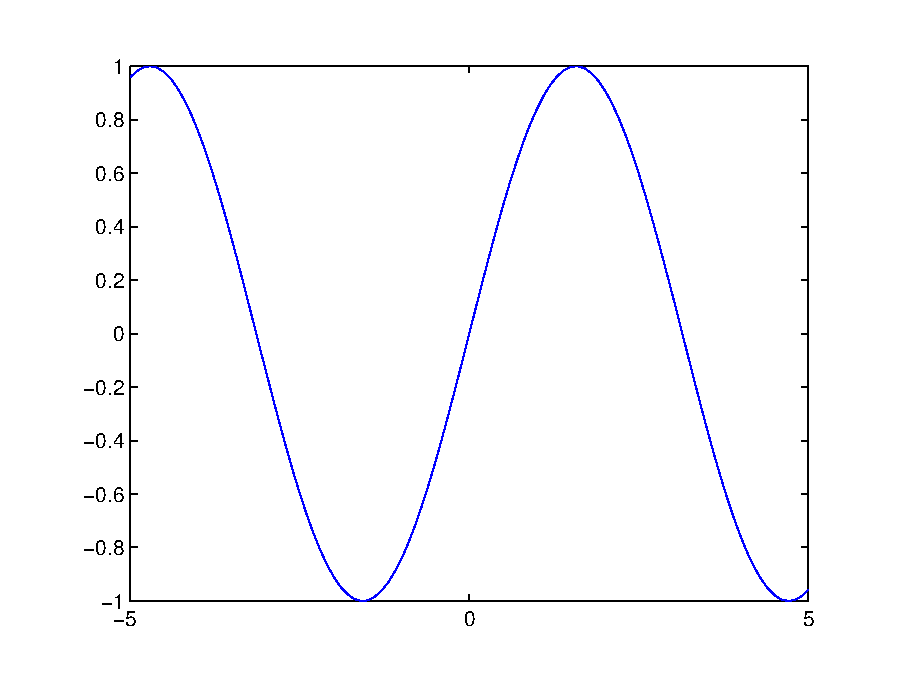
\includegraphics[width=0.95\linewidth]{slike/plot_sin_1.eps}
\caption{Graf funkcije sinus na intervalu $[-5, 5]$.}
\label{fig:plot_sin_1}
\end{figure}

\begin{figure}[!htb]
\centering
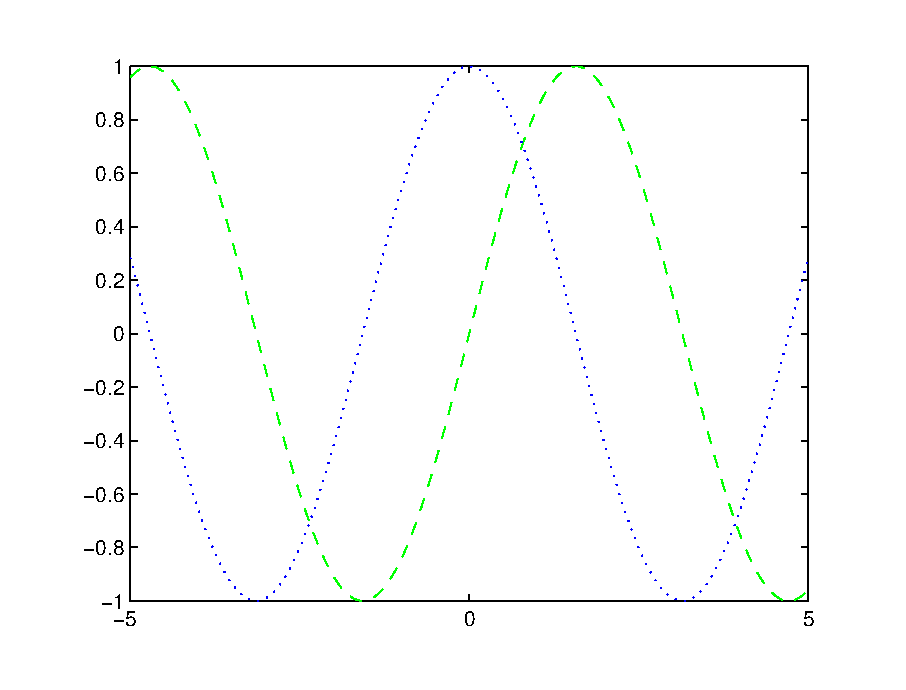
\includegraphics[width=0.95\linewidth]{slike/plot_sin_cos_1.eps}
\caption{Graf funkcija sinus i kosinus na intervalu $[-5, 5]$.}
\label{fig:plot_sin_cos_1}
\end{figure}

\begin{figure}[!htb]
\centering
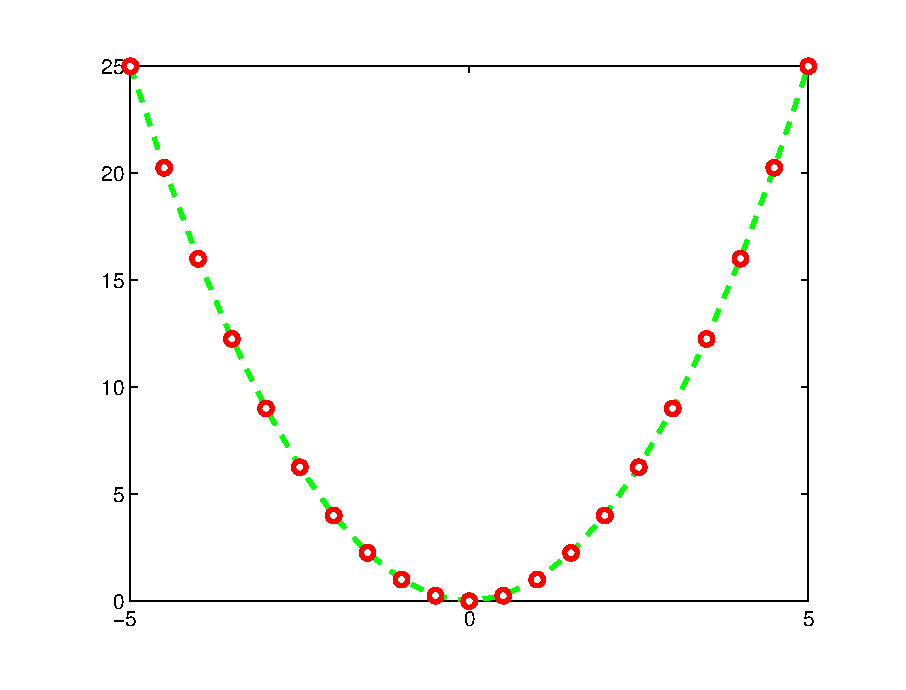
\includegraphics[width=0.95\linewidth]{slike/plot_stil.eps}
\caption{Primjer stiliziranog grafa.}
\label{fig:plot_stil}
\end{figure}

\begin{figure}[!htb]
\centering
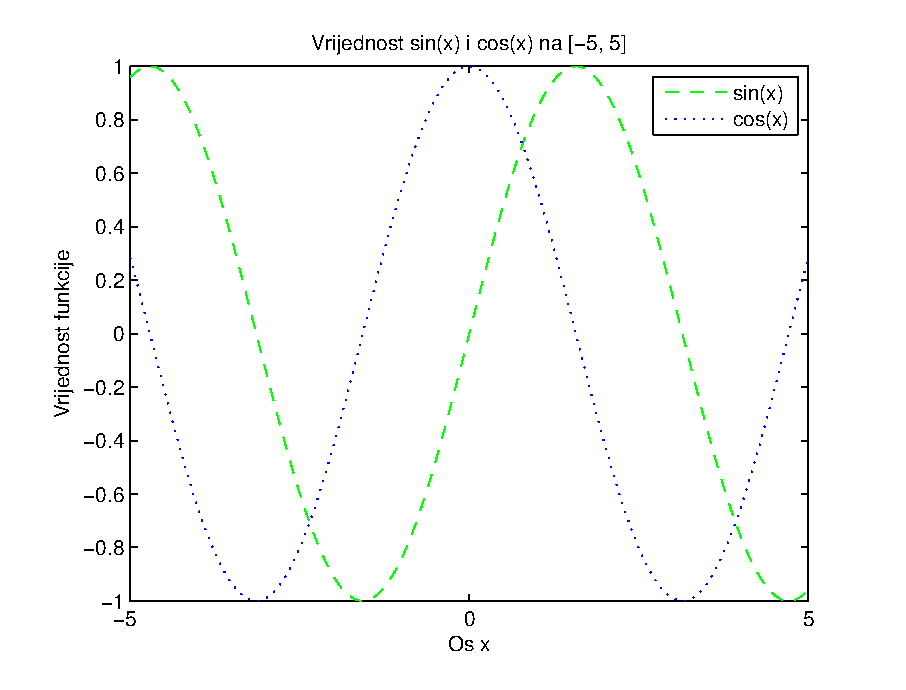
\includegraphics[width=0.95\linewidth]{slike/plot_sin_cos_oznaceno.eps}
\caption{Označeni graf funkcija sinus i kosinus na intervalu $[-5, 5]$.}
\label{fig:plot_sin_cos_oznaceno}
\end{figure}

\begin{figure}[!htb]
\centering
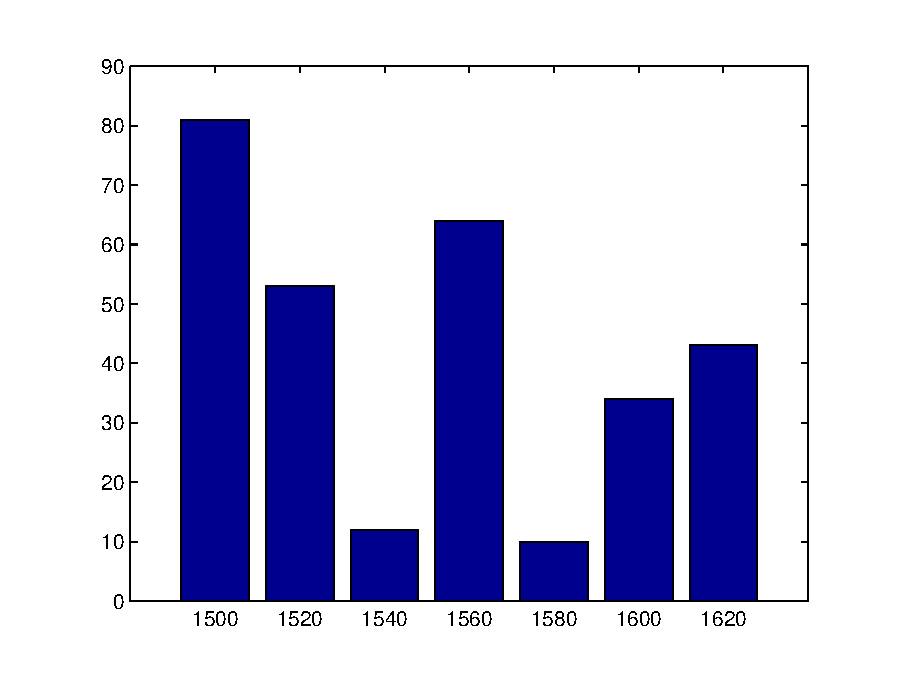
\includegraphics[width=0.95\linewidth]{slike/bar_1.eps}
\caption{Primjer stupčastog grafa.}
\label{fig:bar_1}
\end{figure}

\begin{figure}[!htb]
\centering
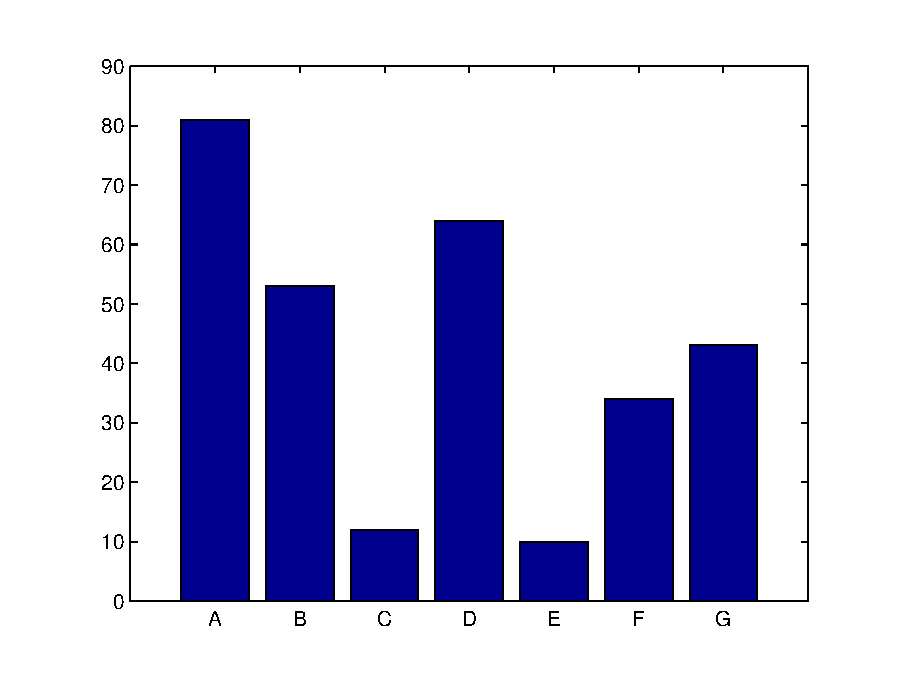
\includegraphics[width=0.95\linewidth]{slike/bar_imenovan.eps}
\caption{Primjer stupčastog grafa sa proizvoljnim imenima stupaca.}
\label{fig:bar_imenovan}
\end{figure}

\clearpage % kako bi sljedeća slika bila na vrhu stranice

\begin{figure}[H]
\centering
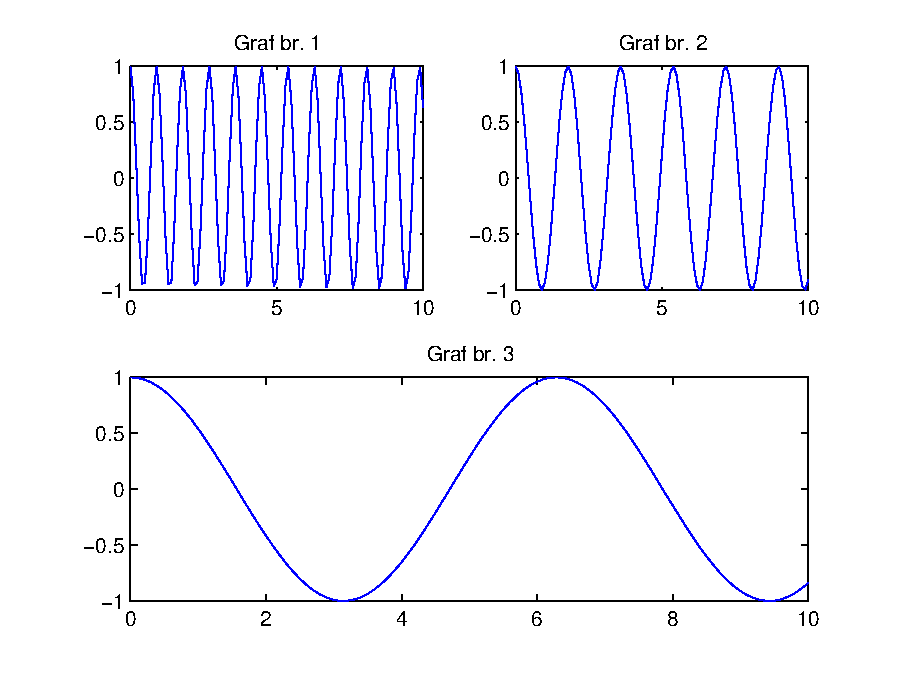
\includegraphics[width=0.95\linewidth]{slike/subplot.eps}
\caption{Primjer više grafova na jednoj slici.}
\label{fig:subplot}
\end{figure}

%\clearpage
%\listoffigures

\end{document}